\section{第2章}


\subsection{题目1}

求方程$2x^2+x-15=0$的正根($x^*=2.5$)近似值,分别用如下三种格式编程计算:

\begin{itemize}
	\item $x_{k+1}=15-x_k^2,k=0,1,2,\cdots$取初始值$x_0=2$
	\item $x_{k+1}=\frac{15}{2x_k+1},k=0,1,2,\cdots$取初始值$x_0=2$
	\item $x_{k+1}=x_k-\frac{2x_k^2+x_k-15}{4x_k+1},k=0,1,2,\cdots$取初始值$x_0=2$
\end{itemize}

依次计算$x_1,x_2,\cdots,x_k,\cdots,$并作图观察解的稳定性、收敛性并分析其原因

\paragraph{不动点法}

设含有n个未知数与n个方程的非线性方程组为F(x)=0,然后把方程组改为便于迭代的等价形式$x=\phi (x)$,由此就可以构造出不动点迭代法的迭代公式为$x_k+1=\phi (x_k)$,如果得到的序列$\{x_k\}$满足$\lim\limits_{k\to \infty} x_k = x^*$,则$x^*$就是$\phi$的不动点,这样就可以求出非线性方程组的解

\paragraph{求解}

直接使用Python对于题目中的三种表达进行计算。

首先,我们对\[x_{k+1}=15-x_k^2,k=0,1,2,\cdots 取初始值x_0=2 \]进行计算。

前四次的迭代结果依次为:\[
x_1=11 \]\[ x_2=-106 \]\[ x_3=-11221 \]\[ x_4=-125910826
\]将前4次的结果作成图像进行观察:
\begin{figure}[H]
	\centering
	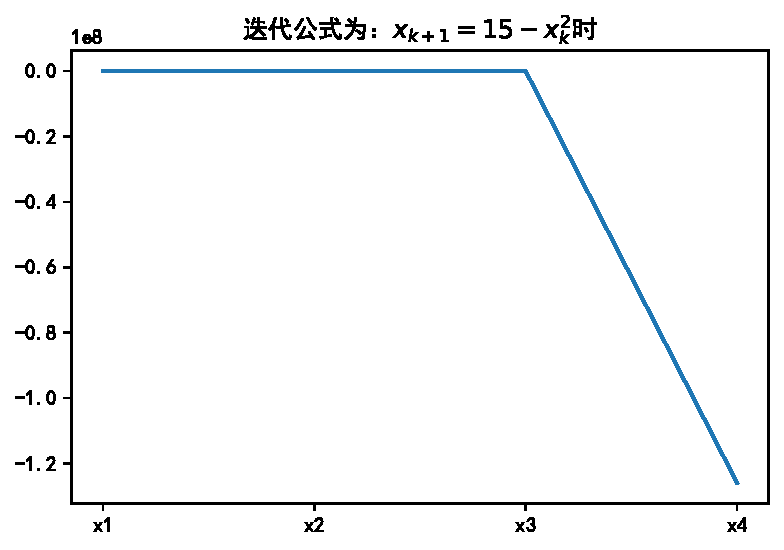
\includegraphics[width=0.7\linewidth]{2-1-1.pdf}
	\caption{}
	\label{fig:2-1-1}
\end{figure}

\paragraph{分析}

由该结果可知,当原方程转换为$x_{k+1}=15-x_k^2,k=0,1,2,\cdots$取初始值$x_0=2$时,方程的解发散,即此时无法求出方程的解。\\



我们对\[ x_{k+1}=\frac{15}{2x_k+1},k=0,1,2,\cdots 取初始值x_0=2 \]进行计算。

前50次的迭代结果依次为:\[ x_1=3.0 \]
\[ x_2=2.142857142857143 \]
\[ x_3=2.8378378378378377 \]
\[ x_4=2.2469635627530367 \]
\[ x_5=2.7302873986735445 \]
\[ x_6=2.3217748374586518 \]
\[ x_7=2.6579016512723084 \]
\[ x_8=2.374994799783671  \]
\[ x_9=2.6087003707152228 \]
\[ x_{10}=2.4125837506412577 \]
\[ \cdots  \]
\[ x_{50}=2.4999395640135855 \]
将前50次的结果作成图像进行观察:
\begin{figure}[H]
	\centering
	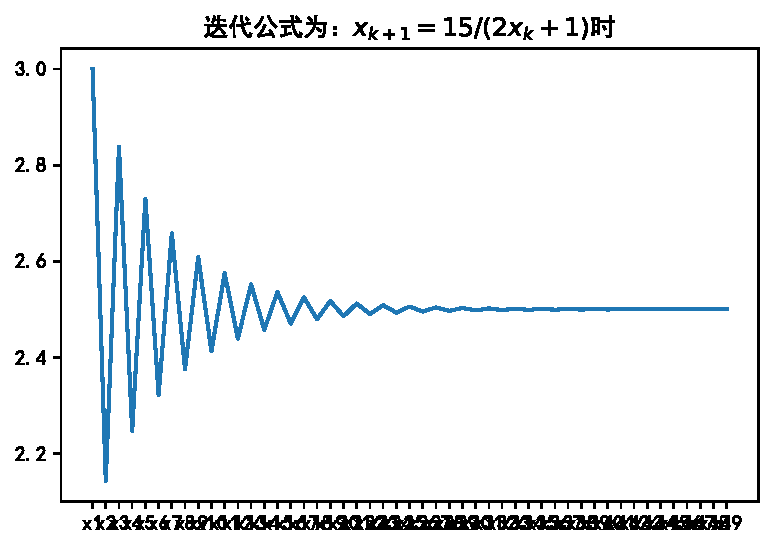
\includegraphics[width=0.7\linewidth]{2-1-2.pdf}
	\caption{}
	\label{fig:2-1-2}
\end{figure}

\paragraph{分析}

由该结果可知,当原方程转换为$x_{k+1}=\frac{15}{2x_k+1},k=0,1,2,\cdots$取初始值$x_0=2$时,方程的解收敛到了2.50,证明该式使用不动点迭代可以得到方程的解。\\


我们对\[ x_{k+1}=x_k-\frac{2x_k^2+x_k-15}{4x_k+1},k=0,1,2,\cdots 取初始值x_0=2 \]进行计算。

前6次的迭代结果依次为:\[ x_{1}=2.5555555555555554 \]
\[ x_{2}=2.5005500550055006 \]
\[ x_{3}=2.5000000550000006 \]
\[ x_{4}=2.5000000000000004 \]
\[ x_{5}=2.5 \]
\[ x_{6}=2.5 \]
将前10次的结果作成图像进行观察:
\begin{figure}[H]
	\centering
	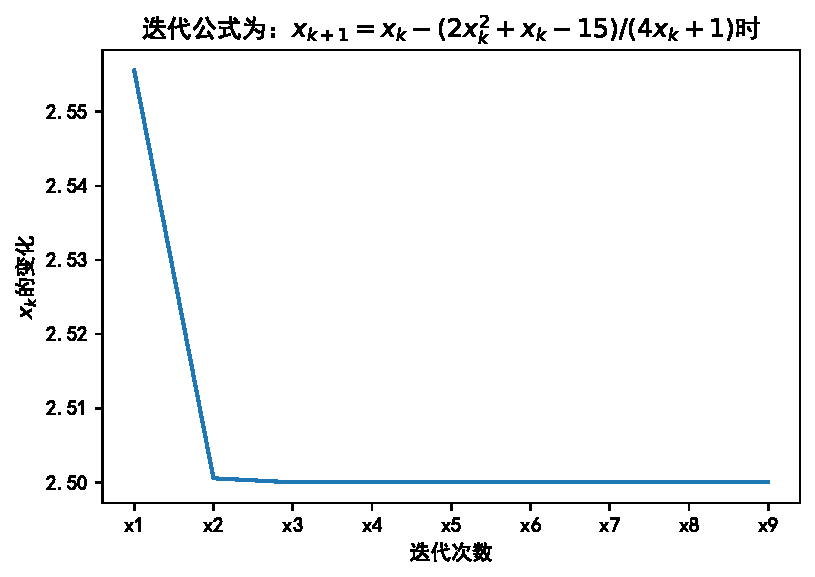
\includegraphics[width=0.7\linewidth]{2-1-3.pdf}
	\caption{}
	\label{fig:2-1-2}
\end{figure}

\paragraph{分析}

由该结果可知,当原方程转换为$x_{k+1}=x_k-\frac{2x_k^2+x_k-15}{4x_k+1},k=0,1,2,\cdots$取初始值$x_0=2$时,方程的解收敛到了2.50,证明该式使用不动点迭代可以得到方程的解。

\subsection{题目2}

证明方程\[2-3x-sin(x)=0\]在$(0,1)$内有且只有一个实根,使用二分法求误差不大于0.0005的根,及其需要的迭代次数。


\paragraph{证明}
~\\
$f(x)=2-3x-sin(x)$\\对f(x)求导,得$f'(x)=-3-cos(x)$\\当$x \in (0,1)$时,$f'(x)<0$,即$f(x)$在(0,1)单调递减\\又,$f(1)=-1-sin(1)<0,f(0)=2>0$\\故可知在(0,1)内,方程在有且只有一个实根


\paragraph{二分法}
~\\
如果$f\in C(a,b)$,且存在数$r\in[a,b]$,满足$f(r)=0$。如果$f(a)f(b)<0$则在区间$[a,b]$内有奇数个零点,若只有一个零点,可以递归用下述方法找到零点:

每次取中点z,若$f(z)=0$,则z就是零点。如果$f(z)f(a)<0$则区间变换到$[a,z]$,否则区间变为$[z,b]$。

从上述递归中容易知道,每次都将零点存在的区间缩小一倍,所以如果在区间$[a,b]$上,如果迭代$n$次,可以得到精度为:
$(b-a)/2^{n+1} $

因此,当$n\rightarrow \infty $的时候,上式右边趋于0,所以得到$r→c_n$,所以只要$n$足够大, 最后一定会收敛到目标点。


\paragraph{求解}

使用二分法进行求解得到根,经过计算,10次迭代后,解收敛,得到解0.505371094。

随迭代次数,解和误差的变化如下表:
\begin{table}[H]
	\centering
	\caption{二分法迭代解和误差的变化}
	\begin{tabular}{lll}
		\hline
		迭代次数 & $x_{mid}$          & 误差                   \\ \hline
		0  & 0.5         & 0.020574461             \\
		1  & 0.75        & -0.93163876             \\
		2  & 0.625       & -0.460097273            \\
		3  & 0.5625      & -0.220802674            \\
		4  & 0.53125     & -0.100361455            \\
		5  & 0.515625    & -0.039953686            \\
		6  & 0.5078125   & -0.009704452            \\
		7  & 0.50390625  & 0.005431321             \\
		8  & 0.505859375 & -0.00213749             \\
		9  & 0.504882813 & 0.001646685             \\
		10 & 0.505371094 & -0.0002454600314260591 \\ \hline
	\end{tabular}
\end{table}

\begin{figure}[H]
	\centering
	\caption{二分法求解过程图}
	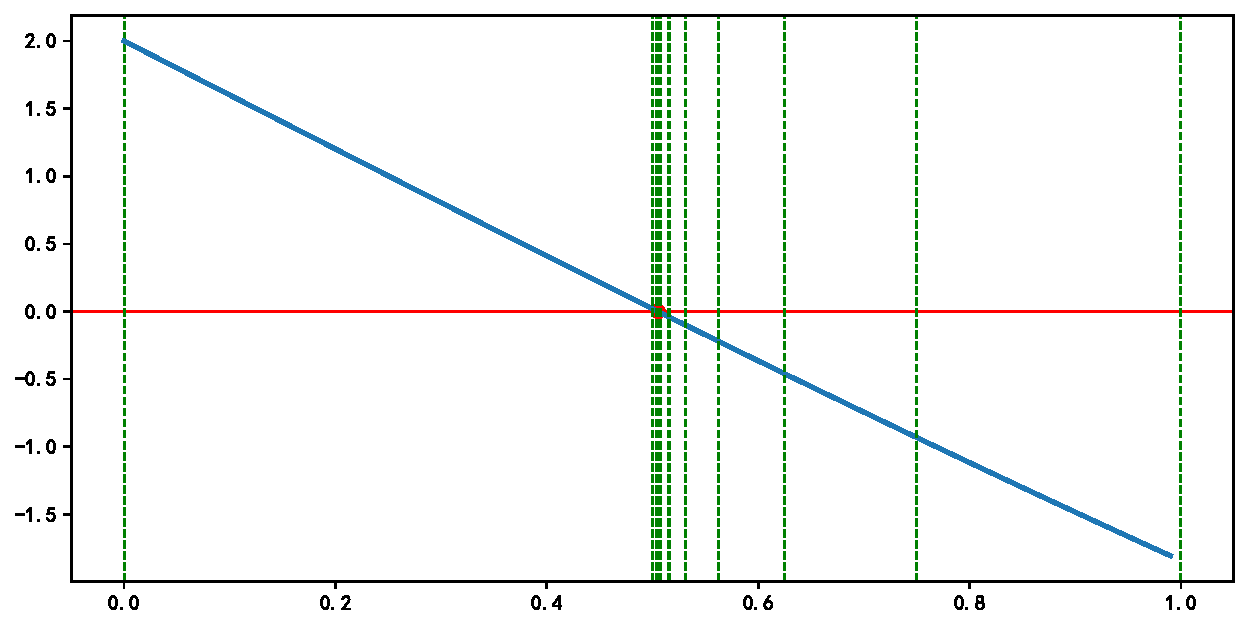
\includegraphics[width=\linewidth]{2-2-1.pdf}
\end{figure}

\paragraph{代码}
~\\
\begin{minted}{python}
def bisection(f, a, b, max_iter, ax=None, px=None):
    if ax is not None:
        ax.axhline(y=0, color='red', linestyle='-', linewidth=1)
        ax.axvline(x=a, linestyle='--', c='green', linewidth=1)
        ax.axvline(x=b, linestyle='--', c='green', linewidth=1)
        ax.plot(px, f(px), linewidth=2)
    if f(a) * f(b) >= 0:
        print("二分法失败.")
        return None
    for _ in range(max_iter):
        c = (a + b) / 2
        if ax is not None:
            ax.axvline(x=c, linestyle='--', c='green', linewidth=1)
        fc = f(c)
        if f(a) * fc < 0:
            b = c
        elif f(b) * fc < 0:
            a = c
        elif fc == 0:
            print("找到准确的解.")
            return c
        else:
            print("二分法失败.")
            return None
    if ax is not None:
        ax.scatter((a + b) / 2, 0, c='red')
    return (a + b) / 2
\end{minted}

\begin{minted}{python}
x = sp.Symbol('x')
f = 2 - 3*x-sp.sin(x)
df = sp.diff(f)
f_eval = sp.lambdify(x, f)
df_eval = sp.lambdify(x, df)
display(Math('f(x) = %s 的导函数为 f^\prime(x) = %s.' % (sp.latex(f), sp.latex(df))))
fig, ax = plt.subplots(nrows=1, ncols=1, figsize=(10, 5))
px = np.arange(0, 1, 0.01)
bisection(f_eval, 0, 1, 10, ax, px)
plt.savefig('2-2-1.pdf', bbox_inches='tight')
\end{minted}


\subsection{题目3}

利用牛顿法求解方程
$$\frac{1}{2}+\frac{1}{4}x^2-x\sin x-\frac{1}{2}\cos2x=0$$
分别取$x_0=\frac{\pi}{2},5\pi,10\pi$,使精度不超过$10^{-5}$,比较初值对计算结果的影响。

\paragraph{牛顿法}
~\\
推导:假设$f\in C^2\left[a,b\right]$, 并且$x^{*}$是$f\left(x \right) = 0$的一个解.

令$\overline{x} \in \left[a,b\right]$是对$x_{*}$的一个近似, 使得$f'\left(\overline{x} \right) \neq 0$且$\left|\overline{x} - x^{*} \right|$比较小. 考虑$f\left(x\right)$在$\overline{x}$处展开的一阶泰勒多项式$f\left(x\right) = f\left(\overline{x} \right) + \left(x - \overline{x}\right) f' \left(\overline{x} \right) + \frac{\left(x-\overline{x}\right)^2}{2}f^{''}\left(\xi \left(x\right) \right)$, 其中$\xi \left(x \right)$在$x$和$\overline{x}$之间. 因为$f\left(x^{*}\right)=0$, 令$x=x^{*}$, 此时有
$0 = f\left(x^{*}\right) = f\left(\overline{x} \right) + \left(x^{*} - \overline{x}\right) f' \left(\overline{x} \right) + \frac{\left(x^{*}-\overline{x}\right)^2}{2}f^{''}\left(\xi \left(x\right) \right)$. 忽略余项, 得到
$0 = f\left(x^{*}\right) \approx f\left(\overline{x} \right) + \left(x^{*} - \overline{x}\right) f' \left(\overline{x} \right)$

求得$$x^{*} \approx \overline{x} - \frac{f\left(\overline{x}\right)}{f'\left(\overline{x}\right)}$$

因此定义迭代序列为:
$x_n = x_{n-1} - \frac{f\left(x_{n-1} \right)}{f'\left(x_{n-1} \right)},\forall n \geq 1$.

\paragraph{求解}
~\\
使用Python的\texttt{sympy包}求得$f(x) = \frac{x^{2}}{4} - x \sin{\left (x \right )} - \frac{1}{2} \cos{\left (2 x \right )} + \frac{1}{2}$ 的导函数为 $$f^\prime(x) = - x \cos{\left (x \right )} + \frac{x}{2} - \sin{\left (x \right )} + \sin{\left (2 x \right )}$$

然后我们做出$f(x) = \frac{x^{2}}{4} - x \sin{\left (x \right )} - \frac{1}{2} \cos{\left (2 x \right )} + \frac{1}{2}$及其导函数的图像进行观察。

\begin{figure}[H]
	\centering
	\caption{$f(x) = \frac{x^{2}}{4} - x \sin{\left (x \right )} - \frac{1}{2} \cos{\left (2 x \right )} + \frac{1}{2}$及其导函数图像}
	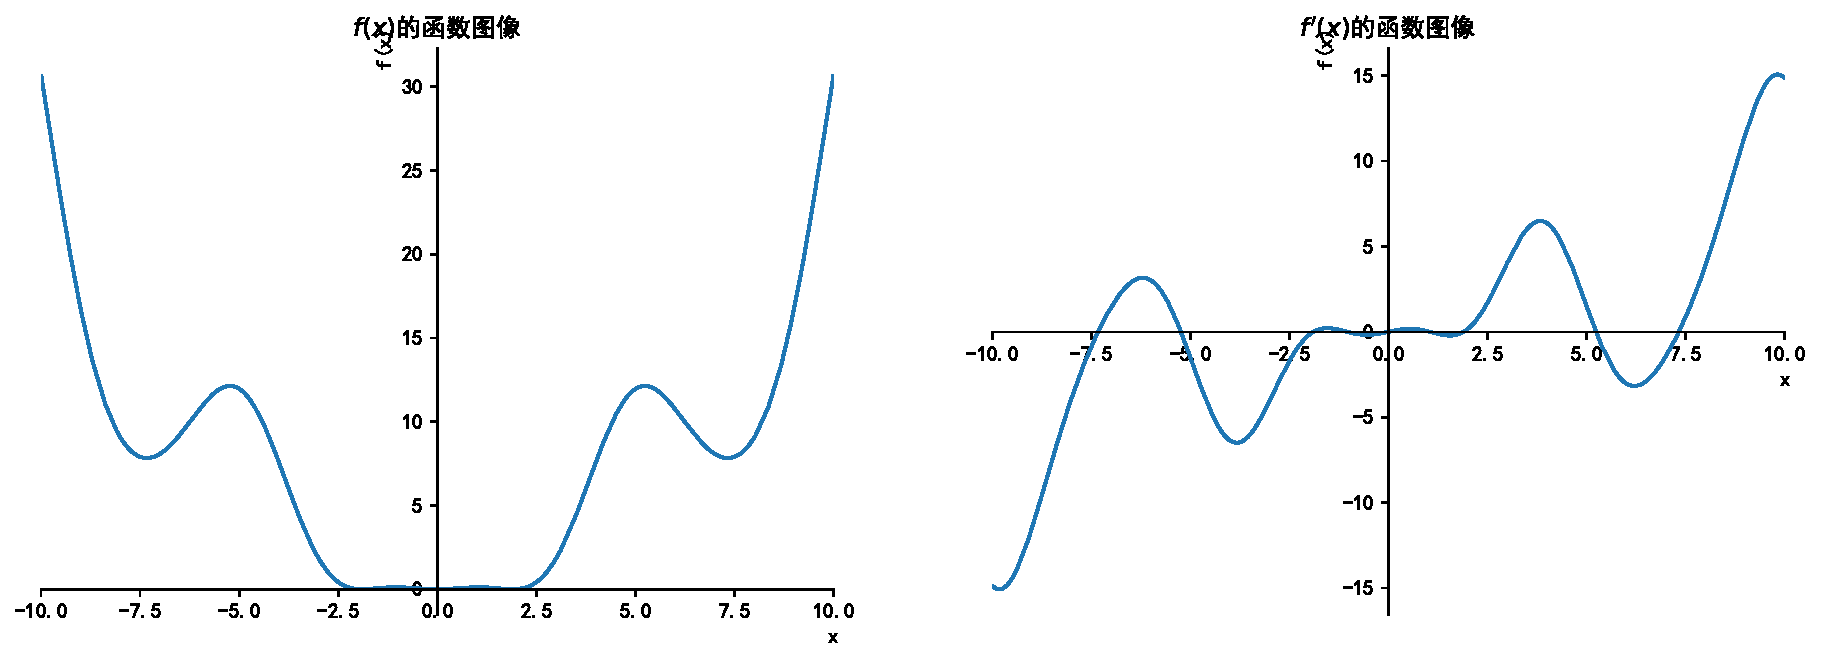
\includegraphics[width=\linewidth]{fig4.pdf}
\end{figure}


观察图像可知,函数零点在$(-2, 2)$这段区间上,因此我们将其放大进行观察:

\begin{figure}[H]
	\centering
	\caption{$f(x)$在$(-2, 2)$区间上的放大图}
	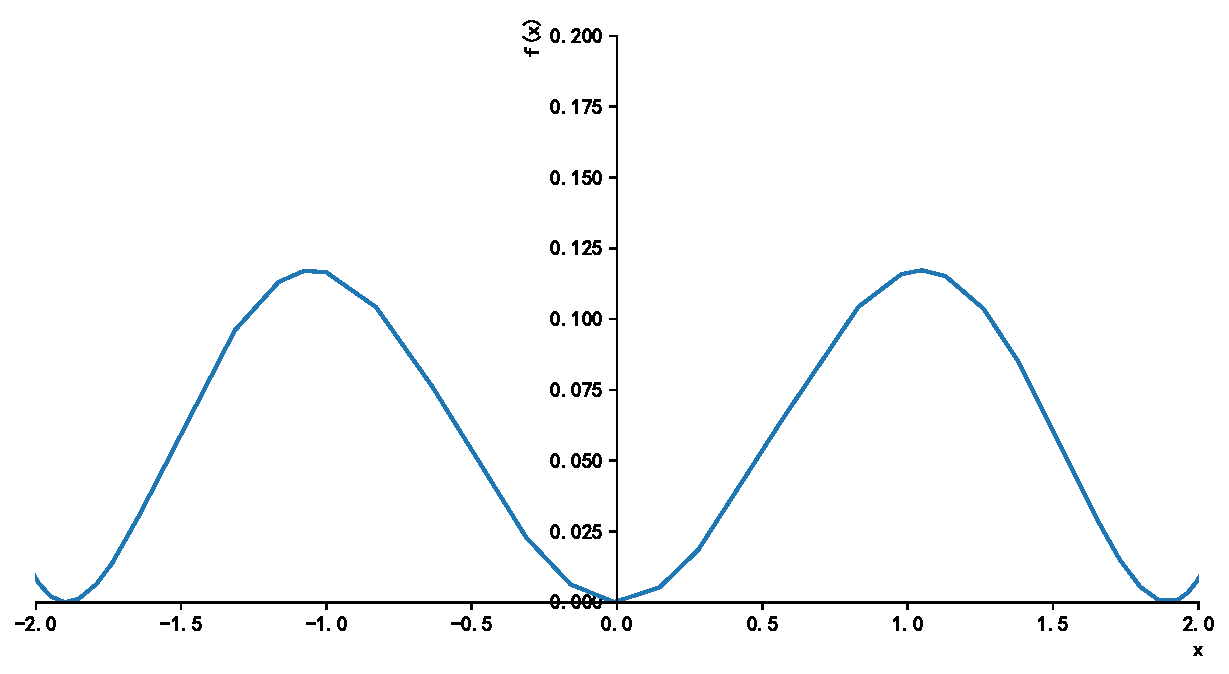
\includegraphics[width=\linewidth]{fig5.pdf}
\end{figure}

然后使用牛顿法求解方程,分别取$x_0=\frac{\pi}{2},5\pi,10\pi$。

\paragraph{$x_0=\frac{\pi}{2}$时} 在6次迭代后找到零点\[x = 1.8924896245342444\]

\begin{figure}[H]
	\centering
	\caption{$x_0 = \pi / 2$ 时牛顿法的过程图}
	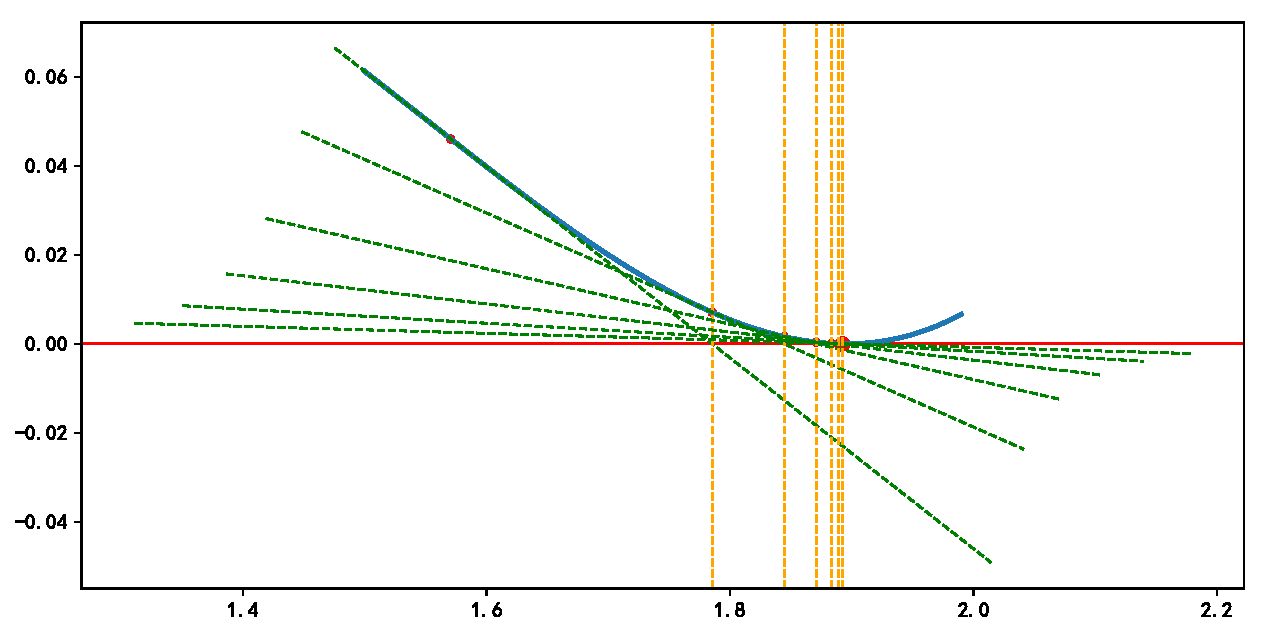
\includegraphics[width=\linewidth]{fig6.pdf}
\end{figure}

\paragraph{$x_0=5\pi$时} 在10次迭代后找到零点\[x = 1.8927898018266247\]

\begin{figure}[H]
	\centering
	\caption{$x_0 = 5\pi$ 时牛顿法的过程图}
	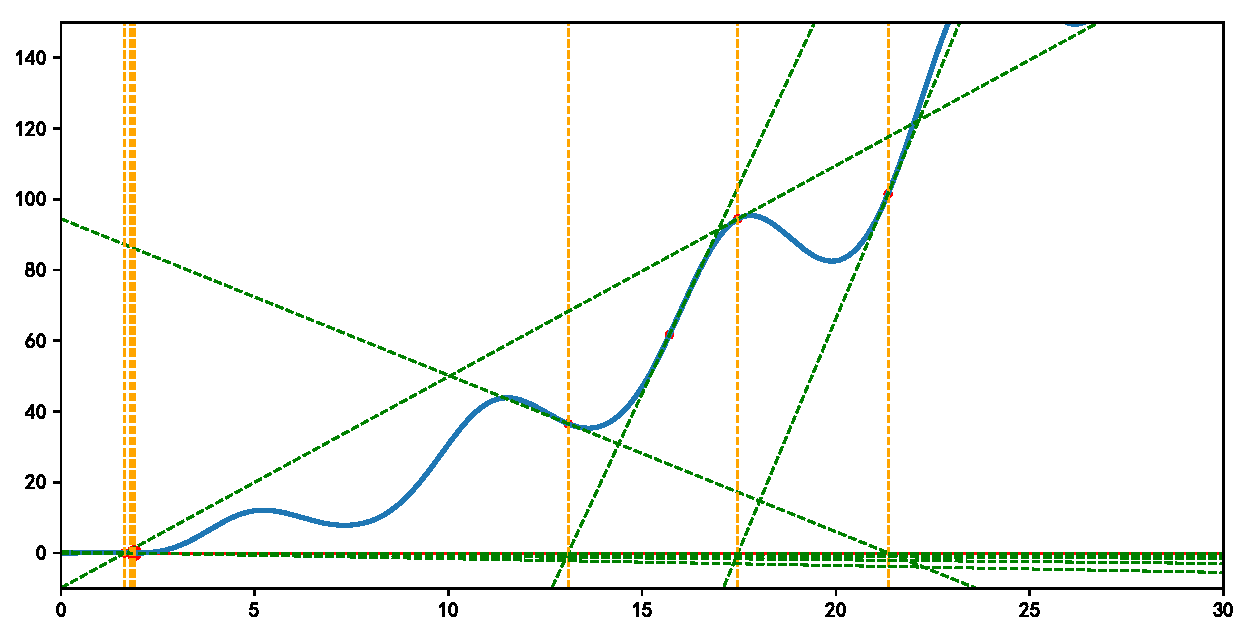
\includegraphics[width=\linewidth]{fig7.pdf}
\end{figure}

\paragraph{$x_0=10\pi$时} 在10313次迭代后找到零点\[x = 1.898094316843809\]

由于当$x_0=10\pi$时时迭代次数过多,计算量过大,所以难以将计算过程进行可视化,仅计算其结果,不进行可视化。

\paragraph{代码}
~\\
\begin{minted}{python}
def newton(f, df, x0, eps, max_iter, ax=None, px=None):
    x = x0
    if ax is not None:
        ax.axhline(y=0, color='red', linestyle='-', linewidth=1)
        ax.plot(px, f(px), linewidth=2)
\end{minted}
\begin{minted}{python}
    for n in range(max_iter):
        fx = f(x)
        if ax is not None:
            ax.scatter(x, fx, c='red', marker='.')
        if abs(fx) < eps:
            print('在%d次迭代后找到解.' % n)
            if ax is not None:
                ax.scatter(x, fx, c='red')
            return x
        dfx = df(x)
        if ax is not None:
            abline(ax, x, fx, dfx)
        if dfx == 0:
            print('导数值为0,无法找到解.')
            return None
        x = x - fx / dfx
        if ax is not None:
            ax.axvline(x=x, linestyle='--', c='orange', 
                       linewidth=1)
    print('超过最大迭代次数,无法找到解.')
    return None
    
px = np.arange(1.5, 2.0, 0.01)
display(Math('找到零点x = %s.' % 
  newton(f_eval, df_eval, np.pi / 2, 1e-5, 100, ax, px)))
px = np.arange(0, 30, 0.1)
plt.xlim(0, 30)
plt.ylim(-10, 150)
display(Math('找到零点x = %s.' %
  newton(f_eval, df_eval, 5 * np.pi, 1e-5, 100, ax, px)))
display(Math('找到零点x = %s.' %
  newton(f_eval, df_eval, 10 * np.pi, 1e-5, 20000)))
\end{minted}

\paragraph{解与迭代次数的关系探究}
~\\
下面对解和迭代次数的关系进行探究(以初值$x_0 = \frac{\pi}{2}$为例):

\begin{figure}[H]
	\centering
	\caption{解与迭代次数的关系图}
	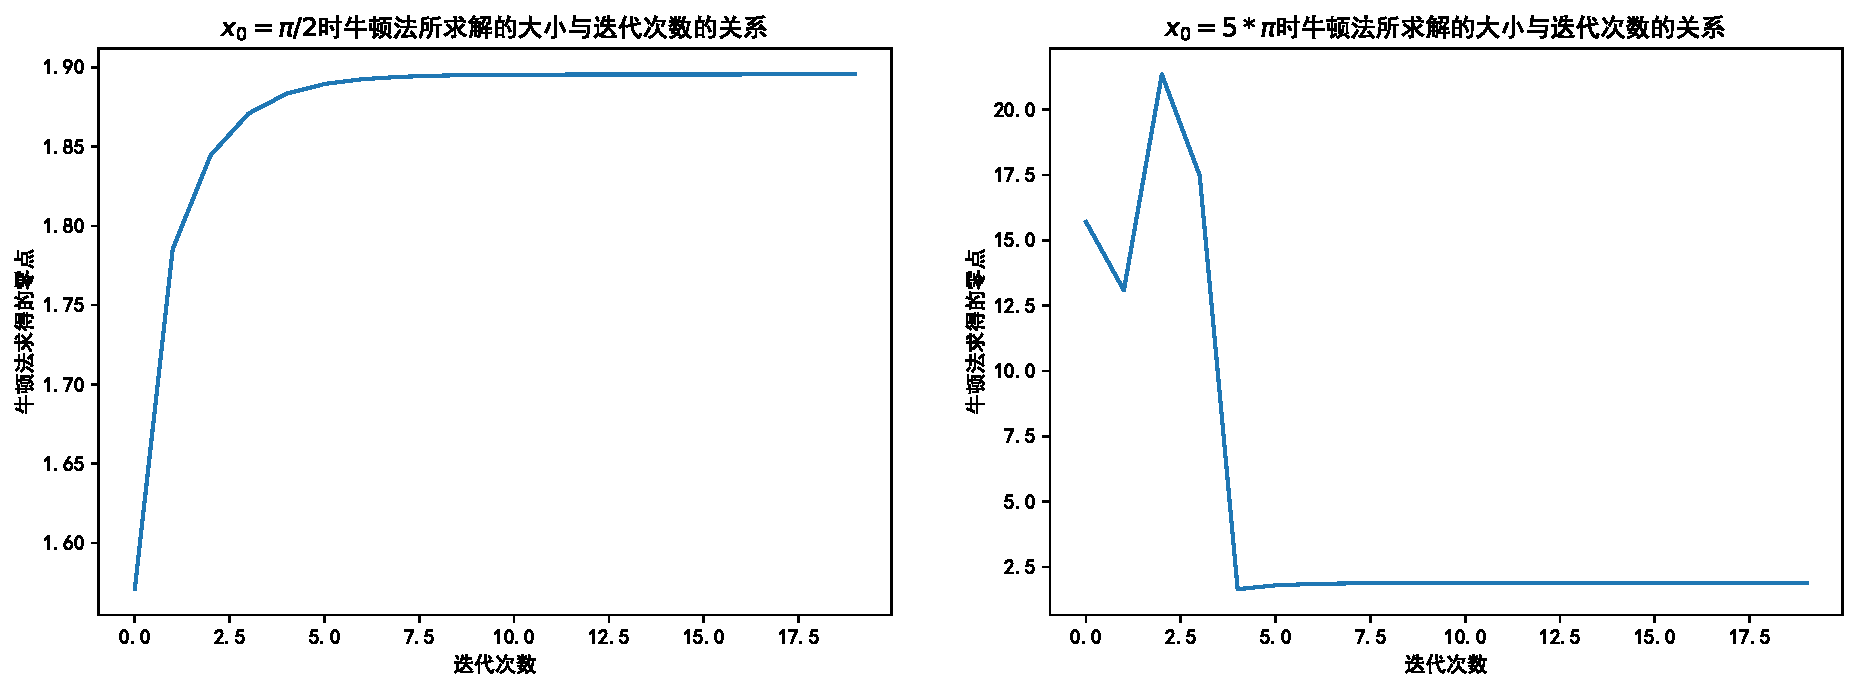
\includegraphics[width=\linewidth]{fig8.pdf}
\end{figure}

随着迭代次数的增加,解的大小的绝对量变化越来越小;初值的选择对于迭代的次数与解的质量有很大关系。

\subsection{题目4}

已知$$f\left(x\right) = 5x - e^x$$
在$\left(0,1\right)$之间有一个实根,试分别用二分法、牛顿法、割线法、错位法设计相应的计算格式,并编程求解。

\paragraph{二分法}
~\\
如果$f\in C(a,b)$,且存在数$r\in[a,b]$,满足$f(r)=0$。如果$f(a)f(b)<0$则在区间$[a,b]$内有奇数个零点,若只有一个零点,可以递归用下述方法找到零点:

每次取中点z,若$f(z)=0$,则z就是零点。如果$f(z)f(a)<0$则区间变换到$[a,z]$,否则区间变为$[z,b]$。

从上述递归中容易知道,每次都将零点存在的区间缩小一倍,所以如果在区间$[a,b]$上,如果迭代$n$次,可以得到精度为:
$(b-a)/2^{n+1} $

因此,当$n\rightarrow \infty $的时候,上式右边趋于0,所以得到$r→c_n$,所以只要$n$足够大, 最后一定会收敛到目标点。

\paragraph{求解}
~\\
使用二分法进行求解得到根$0.25917110181907377$

\begin{figure}[H]
	\centering
	\caption{二分法求解过程图}
	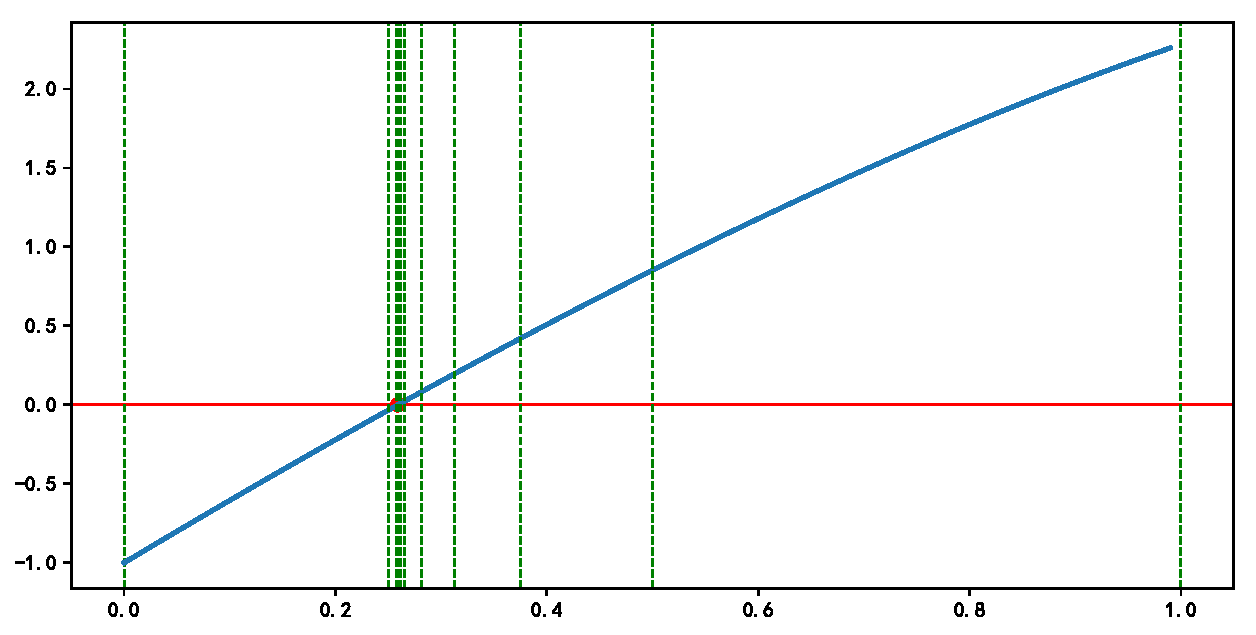
\includegraphics[width=\linewidth]{fig9.pdf}
\end{figure}

\paragraph{二分法代码}
~\\
\begin{minted}{python}
def bisection(f, a, b, max_iter, ax=None, px=None):
    if ax is not None:
        ax.axhline(y=0, color='red', linestyle='-', linewidth=1)
        ax.axvline(x=a, linestyle='--', c='green', linewidth=1)
        ax.axvline(x=b, linestyle='--', c='green', linewidth=1)
        ax.plot(px, f(px), linewidth=2)
    if f(a) * f(b) >= 0:
        print("二分法失败.")
        return None
    for _ in range(max_iter):
        c = (a + b) / 2
        if ax is not None:
            ax.axvline(x=c, linestyle='--', c='green', linewidth=1)
\end{minted}
\begin{minted}{python}
        fc = f(c)
        if f(a) * fc < 0:
            b = c
        elif f(b) * fc < 0:
            a = c
        elif fc == 0:
            print("找到准确的解.")
            return c
        else:
            print("二分法失败.")
            return None
    if ax is not None:
        ax.scatter((a + b) / 2, 0, c='red')
    return (a + b) / 2
\end{minted}

\paragraph{牛顿法}
~\\
首先使用Python的\texttt{sympy}包对函数$f\left(x\right) = 5x - e^x$进行求导,得$f(x) = 5 x - e^{x}$的导函数为$ f^\prime(x) = - e^{x} + 5$,然后对其图像进行观察。

\begin{figure}[H]
	\centering
	\caption{$f(x)$与$f^\prime(x)$的函数图像}
	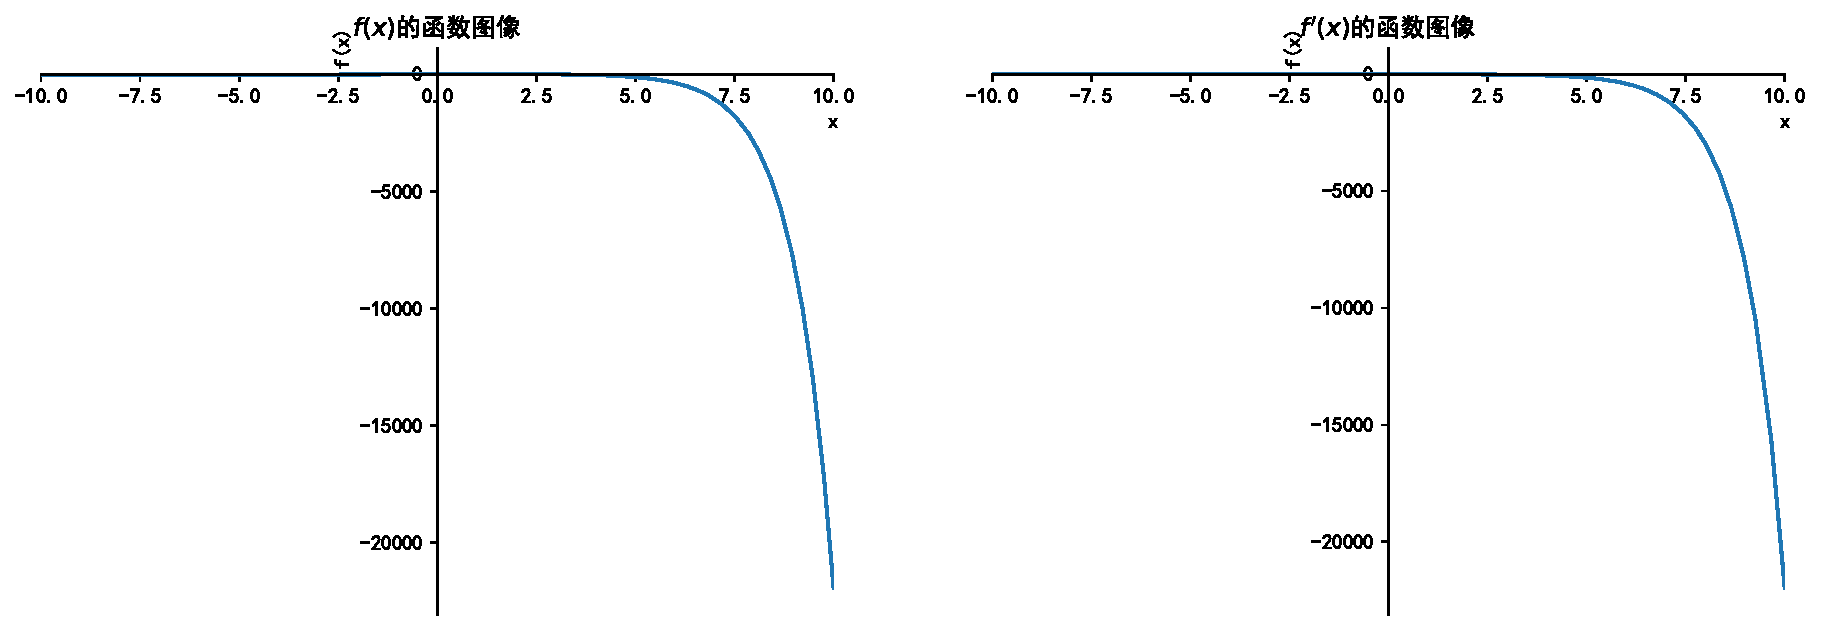
\includegraphics[width=.9\linewidth]{fig_1.pdf}
\end{figure}

运行牛顿法在4次迭代后找到解$0.2591711017819102$。

\begin{figure}[H]
	\centering
	\caption{牛顿法过程图}
	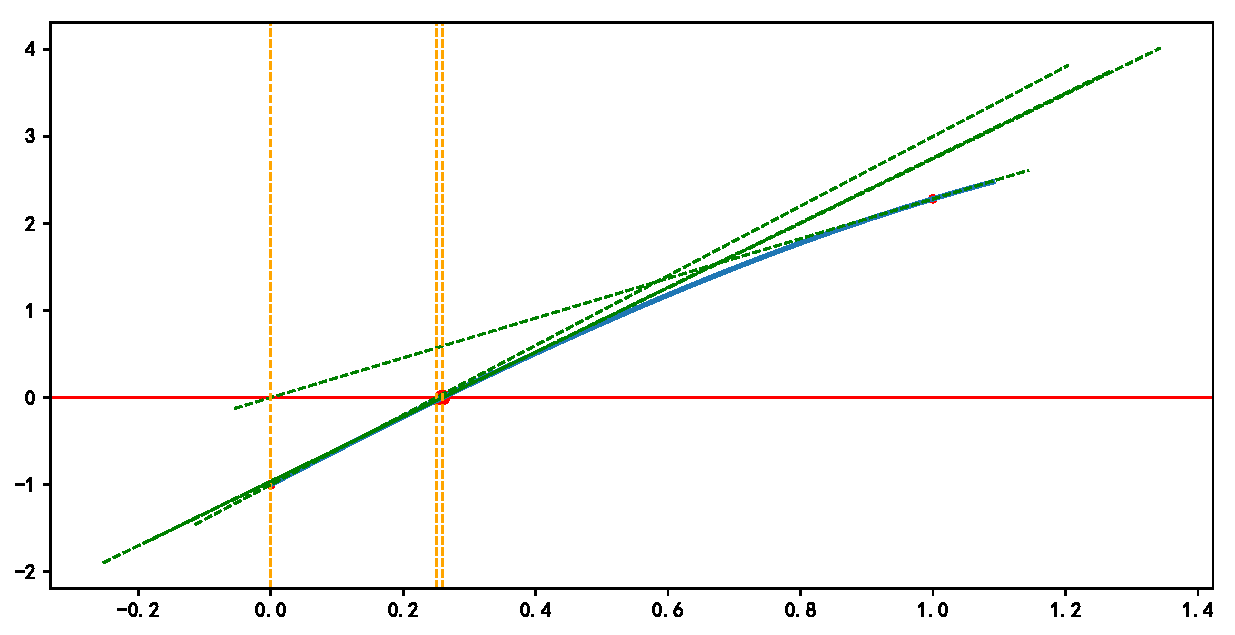
\includegraphics[width=.87\linewidth]{fig10.pdf}
\end{figure}

\paragraph{牛顿法代码}

牛顿法代码请见题目1。

\begin{minted}{python}
px = np.arange(0, 1.1, 0.01)
newton(f_eval, df_eval, 1, 1e-5, 100, ax, px)
\end{minted}
 
\paragraph{割线法}
~\\
推导: 用割线近似代替牛顿法中的切线.

得到公式$x_{k+1} = x_k - f\left(x_k\right) \frac{x_k - x_{k-1}}{f\left(x_k\right) - f\left( x_{k-1}\right)}$。

运行割线法找到解$0.25917110181907377$。

\begin{figure}[H]
	\centering
	\caption{割线法过程图}
	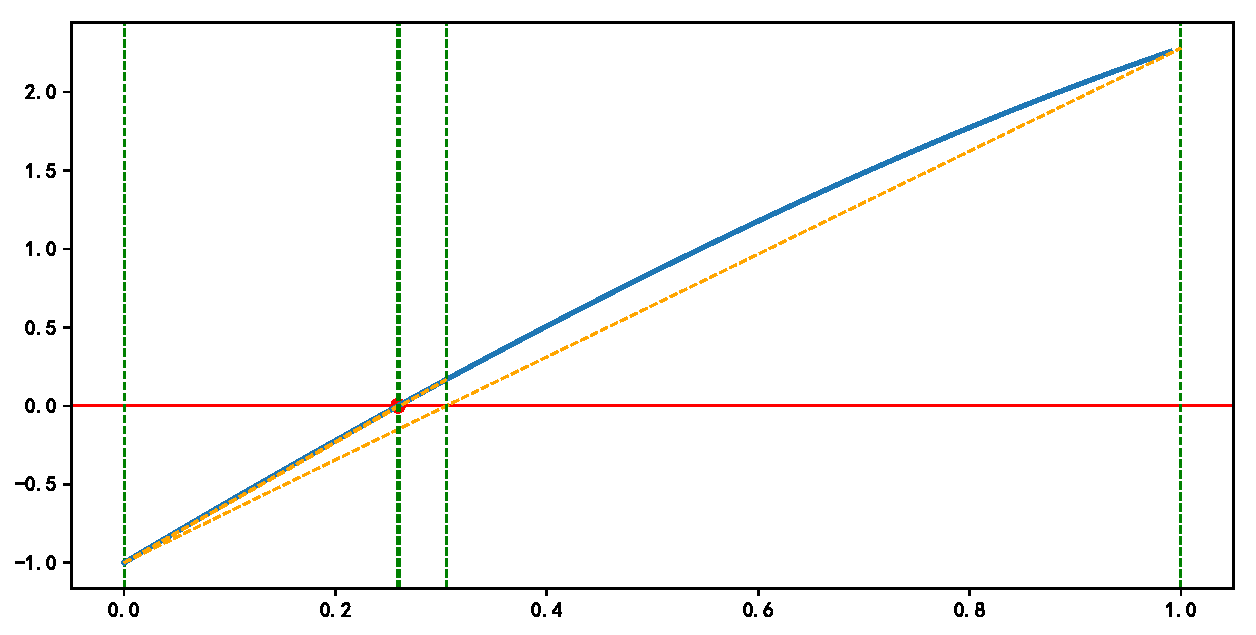
\includegraphics[width=.87\linewidth]{fig11.pdf}
\end{figure}

\paragraph{割线法代码}
~\\
\begin{minted}{python}
def secant(f, a, b, max_iter, ax=None, px=None):
    if ax is not None:
        ax.axhline(y=0, color='red', linestyle='-', linewidth=1)
        ax.axvline(x=a, linestyle='--', c='green', linewidth=1)
        ax.axvline(x=b, linestyle='--', c='green', linewidth=1)
        ax.plot(px, f(px), linewidth=2)
    if f(a) * f(b) >= 0:
        print("割线法失败.")
        return None
    for _ in range(max_iter):
        fa, fb = f(a), f(b)
        c = a - fa * (b - a) / (fb - fa)
        if ax is not None:
            ax.plot([a, b], [fa, fb], c='orange', linestyle='--', 
                    linewidth=1)
            ax.axvline(x=c, linestyle='--', c='green', linewidth=1)
        fc = f(c)
        if fa * fc < 0:
            b = c
        elif fb * fc < 0:
            a = c
        elif fc == 0:
            print("找到准确的解.")
            return c
        else:
            print("割线法失败.")
            return None
    if ax is not None:
        ax.scatter(a - f(a) * (b - a) / (f(b) - f(a)), 0, c='red')
    return a - f(a) * (b - a) / (f(b) - f(a))
\end{minted}

\paragraph{错位法}
~\\
推导:要在区间$\left[p_0,p_1 \right]$上寻找$f\left(x\right) = 0$的解, 其中$f\left(p_0 \right) f\left(p_1 \right) < 0$.

使用与切线法相同的方式, 找到近似点$p_2$.

为确定使用哪一条线计算$p_3$, 计算$f\left(p_2 \right) f\left(p_1 \right)$和$f\left( p_2\right) f\left(p_0 \right)$.

如果$f\left(p_2 \right) f\left(p_1 \right) < 0$, 说明$p_1,p_2$中间包含了一个根, 那么取$\left(p_1,f\left(p_1\right) \right),\left(p_2,f\left(p_2 \right)\right)$线段的斜率, 作为切线法中的斜率.

运行错位法找到解$0.25917110181907377$。

\begin{figure}[H]
	\centering
	\caption{错位法过程图}
	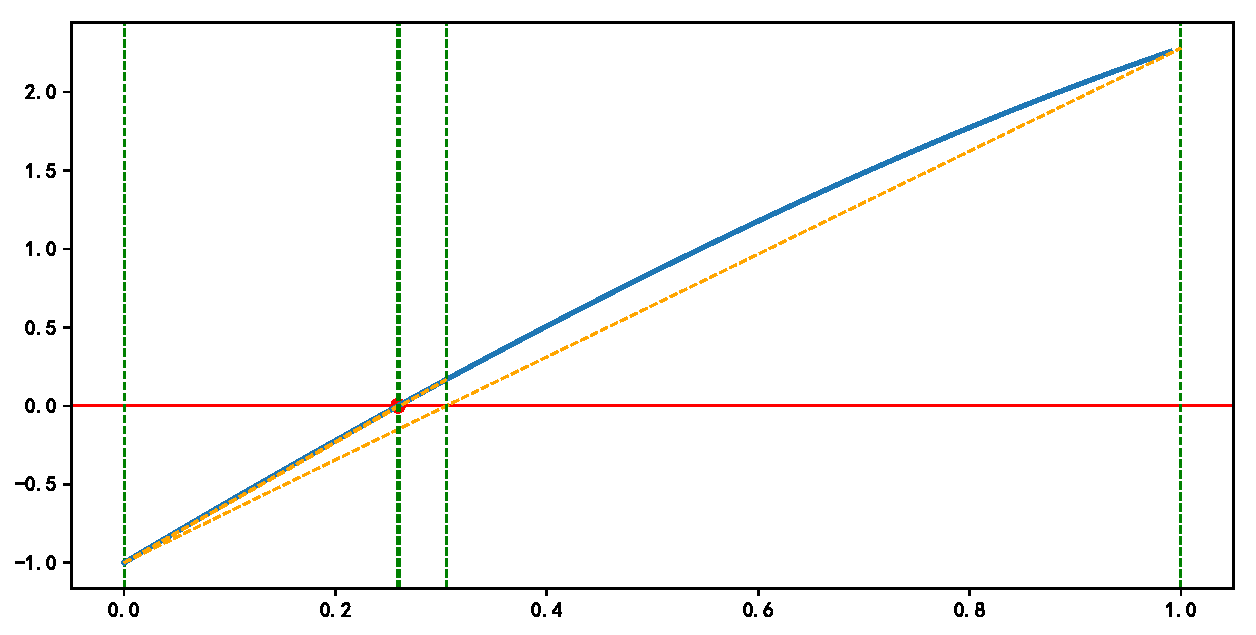
\includegraphics[width=\linewidth]{fig12.pdf}
\end{figure}

\paragraph{错位法代码}
~\\
\begin{minted}{python}
def secant(f, a, b, max_iter, ax=None, px=None):
    if ax is not None:
        ax.axhline(y=0, color='red', linestyle='-', linewidth=1)
        ax.axvline(x=a, linestyle='--', c='green', linewidth=1)
        ax.axvline(x=b, linestyle='--', c='green', linewidth=1)
        ax.plot(px, f(px), linewidth=2)
    if f(a) * f(b) >= 0:
        print("割线法失败.")
        return None
\end{minted}
\begin{minted}{python}
    for _ in range(max_iter):
        fa, fb = f(a), f(b)
        c = a - fa * (b - a) / (fb - fa)
        if ax is not None:
            ax.plot([a, b], [fa, fb], c='orange', linestyle='--', 
                    linewidth=1)
            ax.axvline(x=c, linestyle='--', c='green', linewidth=1)
        fc = f(c)
        if fa * fc < 0:
            b = c
        elif fb * fc < 0:
            a = c
        elif fc == 0:
            print("找到准确的解.")
            return c
        else:
            print("割线法失败.")
            return None
    if ax is not None:
        ax.scatter(a - f(a) * (b - a) / (f(b) - f(a)), 0, c='red')
    return a - f(a) * (b - a) / (f(b) - f(a))

fig, ax = plt.subplots(nrows=1, ncols=1, figsize=(10, 5))
px = np.arange(0, 1, 0.01)
regula(f_eval, 0, 1, 100, ax, px)
\end{minted}